  \mysection{Fighting}{combat-fighting}

  \callout {
  \mybullet {
    \item Combat is conflict that takes place between \mylink{Adventurers}{roles-adventurer} and \mylink{Monsters}{roles-monster} at a particular \mylink{Distance}{game-distance}.

    \item Combat consists of \mylink{Moments}{time-combat} and takes \mylink{Minutes}{time-combat} to complete. 

    \item Each Moment you make an \mylink{Init}{combat-init} try to determine how many Actions you get.  If you \RO, you get 2 Actions; otherwise, you get 1 Action.

    \item If you have 2 Actions, you can take 1 \mybold{before} the Monsters' turn and one \mybold{after} the Monsters' turn. If you have 1 Action, you can only take it \mybold{after} the Monsters' turn.

    \item There are 2 kinds of Actions: Maneuver Actions and Combat Actions.  \mybold{If you take a Combat Action, your Moment ends}.

    \item Certain Actions occur at the \mylink{Top or Bottom of the Moment}{time-combat}.
  }}



  \mysubsection{Who Goes First?}{combat-init}

  The Init try decides whether your Adventurer will take 1 or 2 Actions this Moment. 

Before the Init try is rolled, the Arbiter must determine if one side (your Band, or the Monsters) got \mybold{the Drop} on the other.

\myimage{combat/Fighting1}

\cbreak



  \mysubsection{The Drop}{combat-drop}

  You sneak up on a couple of ogres arguing over who gets to eat which half of Dwight the Unlucky, or you come around the corner right into an ambush. The Arbiter will first determine if either side is \mylink{Surprised}{effect-surprised} (see the section on \mylink{Effects}{game-effects}
 for more info). If the Arbiter determines that you've Surprised the Monster, you get \mybold{the Drop} on them (and if you are Surprised, the Monsters have gotten the Drop on you!).

  If the Monsters get the Drop on you, they get to act for a full Moment before you roll your Init. Any damage you take before you make your Init try \mybold{bypasses \mylink{Grit}{adventurer-flesh-grit}}. If you get the Drop on the Monsters, you get to act for a full Moment before they do. Any damage you deal to the Monsters are \mylink{Crits}{combat-crits-and-fumbles} (deal \MAX damage +4, unless you fail a \RSTRY{\FOC}). 

Additionally, if you have a \mylink{Knave}{trope-knave} or \mylink{Murk}{species-murk} in your Band, the Drop allows them to attempt a \mylink{Murder}{vulgate-whisper-the-bride} by using their knowledge of the \mylink{Whispers of the Bride}{vulgate-whisper-the-bride} (see the section on \mylink{Whispers}{vulgate-whispers} for more details).


    Once the Drop is resolved, all Allies must try their \mybold{Init} at the top of the Moment. If you successfully \RO, you can take 2 Actions (1 \myital{before} the Monsters take their turn, and one \myital{after}); if you aren't able to assemble a 20 in this \RO try, you go \myital{after} the Monsters take their turn. The Init try is your \INT plus your \mylink{Movement Die}{combat-movement-die} plus the \mylink{Monster's Speed}{combat-monster-speed}.


  \formula{Init Try}{
    \RO: \INT \PLUS \MD \PLUS \mybold{Monster Speed}
  } 


\newpage

  \myhighlight{The Movement Die}{combat-movement-die} \MD

  \mylink{Armor}{gear-armor} is great to have if you plan on getting hit, but it has a cost - the heavier and more cumbersome the Armor, the lower your Move Die. Each type of armor has a \MD associated with it:

  \mytable{Y Y}{
    \thead{\mylink{Armor}{gear-armor}} & \thead{\MD} \\
  }{
    None & d20 \\
    Light & d12 \\
    Medium & d8 \\
    Heavy & d4  \\
  }


  \myhighlight{The Monster's Speed}{combat-monster-speed}

  Most Monsters you meet are going to have a speed of d16. Some Monsters are Fast - their speed is d12.  Some Monsters are Slow - their speed is d20.  See the section on \mylink{Monsters}{monsters} for more details.

  \myimage{combat/Combat_1}


\cbreak

  \crunch{Mixed Init}{combat-mixed-init}

  If the Allies are fighting Monsters with mixed speeds (a group of slow blood puppets led by a necromancer who moves at normal speed, say), use Init as follows:



\callout{\footnotesize{
  \mynumlist {
    \item  The Allies roll their Init against the necromancer (d16 speed).  If they \RO, they can take an Action (see below).
    \item  The necromancer takes her turn.
    \item  Any Allies that won Init against the necromancer can take their second Action now.  Any Allies who failed to \RO against the necromancer should now test their Init against the blood puppets.  If they \RO, they can take an Action.
    \item  The blood puppets take their turn.
    \item  Allies who have any Actions left, or Allies who failed both Init tests now take their Action.
  }
}}

\newpage

\end{multicols*}
  \mysubsection{Actions}{combat-actions}

  Combat consists of \mylink{Moments}{time-combat} and takes \mylink{Minutes}{time-combat} to finish. Each Moment you make an \mylink{Init}{combat-init} try to determine how many Actions you get.  If you \RO, you get 2 Actions; otherwise, you get 1 Action.

  If you have 2 Actions, you can take 1 Action \mybold{before} the Monster and 1 Action \mybold{after} the Monster. If you fail, you can only take 1 Action \mybold{after} the Monster. You can always choose to act after - there's no need to roll at that point. You can act as a group and decide your own order for Actions in each Moment. 

  Your Action can be either a \mybold{Maneuver} or \mybold{Combat} Action. Maneuvers (\mylink{Basic}{combat-basic-maneuver} and \mylink{Tactical}{combat-tactical-maneuver}) cover you moving around the battlefield, attending to hurt Allies, getting things out of your pack, setting up attacks, etc. Combat Actions (\mylink{Deeds}{combat-deeds} and \mylink{Attacks}{combat-attack-action}) are actions taken to actually fight with a Monster. You can only take 1 Combat Action every Moment  - taking a Combat Action immediately ends your turn.


  \myctrtable{Y Y}{
    \thead{Maneuver Actions} & \thead{Combat Actions} \\
  }{
    Basic & Deed \\
    Tactical & Attack \\
  }


\vspace{2pt}

\begin{multicols*}{2}

  \mysubsection{Maneuver Actions}{combat-maneuvers}

  \callout {
    Getting better position, pulling something from your pack, etc. Maneuver Actions are divided into \mybold{Basic} and \mybold{Tactical} Maneuvers. Taking a Maneuver Action does \mybold{not} end your Moment.
  }

  \myhighlight{Basic Maneuver}{combat-basic-maneuver}

  Basic Maneuvers involve positioning yourself in combat, readying equipment, picking up something you dropped, etc.  A Basic Maneuver is anything that might take you a handful of seconds to do.  For example:

  \mybullet { 
    \item Move somewhere \mylink{Nearby}{game-distance};  
    \item Ready a shield and/or weapon; 
    \item Switch weapons; 
    \item Pick up something you dropped; 
    \item Get up from the \mylink{Prone}{effect-prone} position; 
    \item Light a torch or flaming oil; 
    \item Grab something out of your pack; 
    \item Drink a potion or applying a salve;
    \item etc.
  }

  Whether or not something qualifies as a Basic Maneuver is up to the Arbiter's discretion.  It's possible that a Basic Maneuver might take multiple Actions. Some examples:

  \mybullet {
    \item Picking a lock while a fight rages around you;
    \item Tying off a rope and swinging into combat;
    \item Running across the room to dig through a fallen Ally's pack;
    \item Trying to find a spell inside a \mylink{Grimoire}{grimoires};
    \item etc.
  }

  The Arbiter should decide how many Actions this will take ("it'll take you a Basic Maneuver to tie off the rope and another Basic Maneuver to swing into Combat"; "it's a Basic Maneuver to move Nearby, another Basic Maneuver to roll him over and open his pack, and a third Basic Maneuver to find that salve of wound binding").

\end{multicols*}
  \myhighlight{Tactical Maneuver}{combat-tactical-maneuver}

  Tactical Maneuvers utilize the environment of the battlefield to positively influence Combat. You can only use one Tactical Maneuver at a time, and you can't "stack" them (you can't \mylink{Aim}{combat-tactical-maneuver-aim} for multiple Moments and stack the bonuses). Unless it says otherwise, bonuses and penalties apply to the next \RO check.


\begin{multicols*}{2}


  \COMBAT [
    Name = Aim,
    Link = combat-tactical-maneuver-aim,
    Desc = Shoot or Throw Weapons Only
  ]
  
  You take careful aim with your weapon.  If your \myital{next} Attack \RO hits, you \mylink{Crit}{combat-crits-and-fumbles} (you still must roll your \FOC). The benefit lasts until you take a Combat Action or something breaks your aim (moving, taking damaging, Guarding, etc).

  \COMBAT [
    Name = Block,
    Link = combat-tactical-maneuver-block,
    Desc = Brawl weapons only
  ]

  Get in a Monster's way and try to get it to attack you.  You can either "pick a fight" with a Monster Close to you, or move somewhere Nearby. Try your \RSTRY{\PRE}.  If you succeed, the Monster will attack you at its next opportunity.

  \COMBAT [
    Name = Brace,
    Link = combat-tactical-maneuver-brace,
    Desc = Polearm or spear only
  ]

  Set your polearm or spear to defend against incoming Monsters.  If a Monster \mylink{Charges}{monster-action-charge} (including Leaping) during its Action, you may immediately take a Combat Action \mybold{before} the Monster attacks (provided you haven't taken a Combat Action already).

\cbreak

  \COMBAT [
    Name = Rage,
    Link = combat-tactical-maneuver-rage,
    Desc = Brawl weapons only
  ]

  You take an Action to be come \mylink{Enraged}{effect-enraged}.  The target of the rage is "the Monsters". If one of your Allies has injured you in this fight, they count as a Monster.

  \COMBAT [
    Name = Reckless,
    Link = combat-tactical-maneuver-reckless,
    Desc = Brawl weapons only
  ]

  You use an Action to aggressively position yourself against the Monsters.  You gain a bonus modifier to your next Attack \RO and a double penalty to your next Guard \RO i.e. take +2 to Attack but -4 to Guard.  You can only gain up to +4/-8 in this way.

  \COMBAT [
    Name = Warding,
    Link = combat-tactical-maneuver-warding,
    Desc = Brawl weapons only
  ]


  You use an Action to defensively position yourself against the Monster.  You gain a bonus modifier to your next Guard \RO and a double penalty to your next Attack \RO i.e. take +2 to Guard but -4 to Attack. You can only gain up to +4/-8 in this way.

\begin{figure*}
\begin{center}
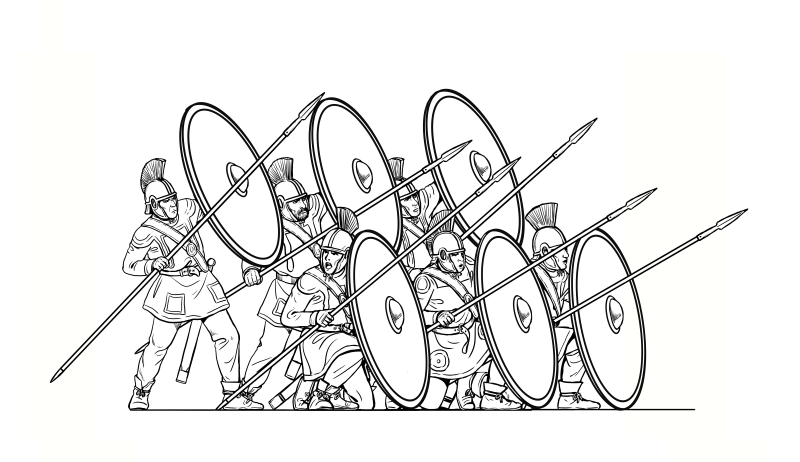
\includegraphics[scale=.4]{combat/CombatShieldWall}
\end{center}
\end{figure*}


\newpage


  \mysubsection{Combat Actions}{combat-combat-actions}

  \callout {
    You commit to your attack and take a Combat Action. Combat Actions are divided into \mybold{Deed} and \mybold{Attack} Actions. Taking a Combat Action \myital{immediately} ends your turn in this Moment.
  }


  \myhighlight{Deeds}{combat-deeds}

  Deeds cover special kinds of attacks you might try to make. You can only use one Deed at a time (you can't use Bum Rush and Florentine at the same time, for example); unless it says otherwise, bonuses and penalties apply to the next \RO check. Deeds are Combat Actions, and taking a Combat Action ends your Moment.

  \COMBAT [
    Name = Bash,
    Link = combat-deeds-bash,
    Desc = Must have a shield equipped (it has to be on your arm / you have to be using it)
  ]

  Get the Monster's attention.  Make an \mylink{Attack try}{combat-attack-action}, but deal damage as if you were \mylink{Unarmed}{combat-damage-unarmed}. If you hit, the Monster will attack you at the next opportunity.


  \COMBAT [
    Name = Bum Rush,
    Link = combat-deeds-bum-rush,
    Desc = Must be attacking with a \VIG Brawl weapon
  ]

  Charge!  Move somewhere Nearby and immediately make an \mylink{Attack try}{combat-attack-action}.

  \COMBAT [
    Name = Disarm,
    Link = combat-deeds-disarm,
    Desc = Brawl weapons only. Your target must be using a 1-handed weapon
  ]

  Make an \mylink{Attack try}{combat-attack-action}.  If your try succeeds, make a \RBONE{\VIG} or \RBONE{\DEX} (your choice) vs. your opponent's \VIG or \DEX (Arbiter's choice). If you win you deal no damage, but your opponent is \mylink{Disarmed}{effect-disarmed}.


  \COMBAT [
    Name = Florentine,
    Link = combat-deeds-florentine,
    Desc = Must be attacking with two Daggers\, two Shortswords\, or a mix of both
  ]

  Make an \mylink{Attack try}{combat-attack-action}. If you hit, roll damage for both weapons and pick the highest:

  \mylist {
    \item  If both dice are natural 1s, you automatically \mylink{Fumble}{combat-crits-and-fumbles}
    \item  If one die is a natural 1, the other die can't Crit (even if you roll \MAX damage)
  }

  \COMBAT [
    Name = Gambit,
    Link = combat-deeds-gambit,
    Desc = Arbiter gets to add penalties to your roll depending on how crazy it is.
  ]

  Called shot. Make an \mylink{Attack}{combat-attack-action}, but roll twice.  If both hit, it happens.  If one hits, it doesn't.  If neither hit, you automatically \mylink{Fumble}{combat-crits-and-fumbles}

  \COMBAT [
    Name = Grapple,
    Link = combat-deeds-grapple,
    Desc = You must be either unarmored or in Light Armor
  ]

  Make an \mylink{Attack try}{combat-attack-action}.  If you succeed, the Monster is grappled. You and the Monster are both considered \mylink{Prone}{effect-prone} until the grapple is broken, meaning Attack and Guard Actions against the Monster get a +4 bonus. However, if an attack against the Monster misses, \RSTRY{\DEX} - a Failure means you are forced to release the Grapple. 

 At the top of the Moment, make an \RB using your \VIG or \DEX (your choice) vs. the Monster's \mylink{Power}{monster-power} or \mylink{Speed}{monster-speed} (Arbiter's choice). If you ever lose the \RB try or take any damage, the grapple is broken.

 Only one Adventurer can grapple a Monster at a time.

  \COMBAT [
    Name = Sunder Shield,
    Link = combat-deeds-sunder,
    Desc = Must have a shield equipped (it has to be on your arm / you have to be using it)
  ]

  If a Monster's attack is about to cause you \mybold{physical} damage, you may immediately destroy your shield, taking no damage. You can wait until after the damage is rolled to decide if you're sundering your shield.  If you already took a Combat Action this Moment, you can't use this Deed.

\cbreak

  \myimage{combat/Combat_2}


  \myhighlight{Attacks}{combat-attack-action}

  \formula{Attack Try}{
    \RO : Weapon Trait \PLUS Monster Weakness \PLUS your Level 
  }

  Eventually your maneuvering and mighty deeds of arms will manifest into a strike at your opponent. The Attack action is when you roll your dice to see if you are able to hit the Monster you're in combat with.

  To see if you hit a Monster, \RO using your weapon's \mylink{Trait}{gear-weapons} plus the Monster's \mylink{Weakness}{monster-weakness}, and add your \LVL to the result. If you fall short, you can try to bump your die roll above a 19 by rolling various other dice (a Sellsword's \mylink{Prowess}{sellsword-prowess}, the associated die of your \mylink{Personality}{adventurer-personality}, etc.).

  If you succeed in your Attack try, you deal damage to the Monster.

\end{multicols*}

  \mysubsection{Dealing Damage}{combat-dealing-damage}

  The damage your weapon does is a single die. Weapon damage is found in the section on \mylink{Weapons}{gear-weapons} under \mylink{Gear}{gear}.  You roll the die and deal that much damage to the Monster.  If you roll a 1, you might Fumble.  If you roll \MAX damage on the die, you might Crit.



  \myhighlight{Crits and Fumbles}{combat-crits-and-fumbles}

  If you roll \MAX damage, your blow may be a Crit. Make a \RSTRY{\FOC} try.  If you roll a Failure, nothing happens. Otherwise, add +4 to your damage.

  If you roll a natural 1 for damage, your blow may be a Fumble. Make a \RSTRY{\FOC} try. If you roll a Failure, you deal no damage to the enemy, and must roll on the table below. The die you use is specified by your \mylink{Armor's}{gear-armor} weight.

  \myctrtable{Y Y}{
    \thead{Weight} & \thead{Die}  \\
  }{
    None & d2  \\
    Light & d4  \\
    Medium & d8 \\
    Heavy & d12 \\  
    Shield & +1 to roll \\
    Helmet & +1 to roll 
  }



If something doesn't apply, move up the chart (that is, things get worse) to the next available effect that works.

\callout{\footnotesize{
\mynumlist {
  \item You miss spectacularly and everyone laughs at you and now no one will invite you to prom.  Lose 1 Grit on account of the shame.
  \item You miss and lose your grip on your weapon and you're holding it all awkward and things feel weird.  Your next Attack try is -4.
  \item You tell everyone that your opponent dodged but really you got all turned around.  Your next Guarding try is -4.
  \item You trip and fall - you are now \mylink{Prone}{effect-prone}.
  \item You \mylink{Disarm}{effect-disarmed} yourself. If it's a Shoot weapon, the bowstring breaks and it'll take Minutes to fix, so let's hope you have a plan B.
  \item If you're wearing a backpack you sever the straps, it splits open, and all the contents spill onto the ground.  Backpack is now useless and everyone can see your weird collection of things you've been stealing.
  \item You really overextend yourself, pull a hammy, and mess up your \mylink{Armor}{gear-armor} (if you're wearing any).  Make an Armor \UD roll.
  \item (or more) Stop hitting yourself!  The damage bypasses your Grit and applies to you instead.
}}}

\newpage
\begin{multicols*}{2}

\myhighlight{Lethal Damage}{combat-damage-lethal}

Certain mighty warriors and terrifying Monsters deal \mybold{Lethal} damage. If they roll \MAX damage, they roll again, adding the second roll to the first. If they roll the \MAX again, they repeat the process. Continue rolling until you do not roll \MAX. Modifiers to damage are added or subtracted \mybold{after} the die explodes (from rolling \mylink{Prowess}{sellsword-prowess}, for instance).

    \example{Charse the Lethal attacks a goblin with a Shortsword (d6).  He rolls his Attack try and hits, and rolls a 6 for damage. He rolls again and rolls another 6.  He rolls a 3rd time and rolls a 4.  He deals 16 points of damage(!) (6+6+4) and the goblin is reduced to a fine pink mist.}


\cbreak

  \myhighlight{Unarmed Damage}{combat-damage-unarmed}

  Your damage for Unarmed combat depends on your \VIG

  \mytable{Y Y}{
    \thead{\VIG} & \thead{Damage} \\
  }{
    d6 & 1  \\
    d8 & 2  \\
    d10 & 3  \\
    etc.
  }

  If you bring someone to 0 Flesh via Unarmed combat, they are \mylink{Knocked Out}{effect-knocked-out} for \DUR{d4}.  Continued Unarmed attacks against Knocked Out foes prompt \DEATH rolls as you beat them to death.

  Note that since this isn't a die roll there's no way to Crit or Fumble.  Fighting unarmed is the same as using a weapon with the \VIG Trait.


